\documentclass[11pt,a4paper,pdftex]{amsart}
\usepackage[psamsfonts]{amssymb}
%\usepackage{amssymb}
\usepackage{amsmath,amsfonts,latexsym}
\usepackage[dvips]{graphicx}
\usepackage{t1enc}
\usepackage[english]{babel}
\usepackage{graphicx}
\usepackage{amscd}
\usepackage{verbatim}
\usepackage{multicol}
\usepackage[utf8]{inputenc}

\newtheorem{ej}{Ejercicio}%[section] %numera os 'Ejercicios' reseteando
%en cada 'cap�tulo'.


\numberwithin{equation}{section}%numera las formulas reseteando
%cada vez que cambia de 'cap�tulo'.

\newcommand{\bej}[1]{\begin{ej}\rm{#1}}
\newcommand{\eej}{\end{ej}\vspace{-0.2cm}}
%---------------------------------------
\newcommand{\be}{\begin{enumerate}}
\newcommand{\ee}{\end{enumerate}}
\newcommand{\bit}{\begin{itemize}}
\newcommand{\eit}{\end{itemize}}
\newcommand{\bc}{\begin{center}}
\newcommand{\ec}{\end{center}}
\newcommand{\ba}{\begin{array}}
\newcommand{\ea}{\end{array}}
\newcommand{\bq}{\begin{quotation}}
\newcommand{\eq}{\end{quotation}}
\newcommand{\beq}{\begin{equation}}
\newcommand{\eeq}{\end{equation}}
\newcommand{\mc}[1]{\mathcal{#1}}
\newcommand{\mb}[1]{\;\mbox{#1}\;}
\newcommand{\su}[1]{\underline{#1}}
\newcommand{\so}[1]{\overline{#1}}
\newcommand{\ang}[1]{\widehat{#1}}
\newcommand{\arc}[1]{\wideparen{#1}}
\newcommand{\cc}{QQ\;}
\renewcommand{\bf}{\textbf}
\newcommand{\comb}[2]{\left(\!\!\!\ba{c}#1\\[1ex]#2 \ea
\!\!\!\right)}
%-----------------------------------------
%conjuntos
\newcommand{\W}{\mathbb W}
\newcommand{\K}{\mathbb K}
\newcommand{\N}{\mathbb N}
\newcommand{\C}{\mathcal C}
\newcommand{\Z}{\mathbb Z}
\newcommand{\Q}{\mathbb Q}
\newcommand{\R}{\mathbb R}
\newcommand{\F}{\mathbb F}
\newcommand{\A}{\mathbb A}
\newcommand{\V}{\mathbb V}
\newcommand{\I}{\mathbb I}
\newcommand{\0}{\mathbb O}
%------------------------------------------
%operaciones
\newcommand{\8}{\infty}
\newcommand{\ie}{\langle}
\newcommand{\de}{\rangle}
\newcommand{\pe}[2]{\ie {#1} \, ; \, {#2} \de }
\newcommand{\f}[1]{\overrightarrow{#1}}
\newcommand{\DT}[2]{\frac{d{#1}}{d{#2}}}
\newcommand{\ds}{\displaystyle}
\newcommand{\dg}{\Delta}
\newcommand{\g}{\nabla}
\newcommand{\D}{\mbox{div}}
\newcommand{\Dp}[1]{\partial_{#1}}
\newcommand{\DP}[2]{\frac{\partial{#1}}{\partial{#2}}}
\newcommand{\sen}[1]{\mbox{sen}\;{#1}}
\newcommand{\Lp}[1]{L^{#1}}
\newcommand{\To}{\longrightarrow}
%-------------------------------------
%griegos
\newcommand{\vi}{\varphi}
\newcommand{\om}{\omega}
\newcommand{\Om}{\Omega}
\newcommand{\ve}{\varepsilon}
%-------------------------
%comandos particulares
\newcommand{\id}[1]{\text{id}_{#1}}
\newcommand{\mD}{\mc{D}}
\newcommand{\mC}{\mc{S}}
\newcommand{\mS}{\mc{SS}}
\newcommand{\mH}{\mc{H}}
\newcommand{\HD}{\mc{H}_\mD}
%%%%%%%%%%%%%%%%%%%%%%%%%%%%%%%%%%%%%%%%%%%%%%%%%%%%%%%%%%%%%%%%%
%Un comando para insertar dibujos
\newcommand{\putfig}[4]{\bigskip \bigskip
             \begin{figure}[ht]
             \epsfxsize=#1cm\hfil{\epsfbox{#2}}
             \caption{#3}
         \label{#4}
             \end{figure}\bigskip}
%La sintaxis
%\putfig{ancho}{.eps}{titulo}{label}
%%%%%%%%%%%%%%%%%%%%%%%%%%%%%%%%%%%%%%%%%%%%%%%%%%%%%%%
%Un comando para insertar dos dibujos
\newcommand{\putfigg}[4]{\bigskip \bigskip
             \begin{figure}[ht]
             \epsfxsize=5cm\hfil{\epsfbox{#1}}
             \epsfxsize=5cm\hfil{\epsfbox{#2}}
             \caption{#3}
         \label{#4}
             \end{figure}\bigskip}
%La sintaxis
%\putfigg{.eps}{.eps}{titulo1}{label1}
%%%%%%%%%%%%%%%%%%%%%%%%%%%%%%
%un dibujo en jpg
\newcommand{\putjpg}[3]{\bigskip
\begin{center}
 \begin{figure}[ht]
  \hspace{5cm}\includegraphics[scale=1.7]{#1.jpg}
  \caption{#2}
  \label{#3}
  \bigskip
  \bigskip
 \end{figure}
\end{center}
}
%la sintaxis \putjpg{.jpg}{Titulo}{label}
%----------------------------------------------------
%diseñoo de la página

\vfuzz7pt % Don't report over-full v-boxes if over-edge is 7pt small
\hfuzz7pt % Don't report over-full h-boxes if over-edge is 7pt small

\pagestyle{myheadings}

\renewcommand{\labelenumi}{({\it \alph{enumi}})}
\renewcommand{\labelenumii}{\arabic{enumii})}

\flushbottom \textwidth17cm \textheight23cm \hoffset=-2cm
\voffset=-0.5cm

\begin{document}


%\markboth{}{\hfil {\sc An\'alisis II--An\'alisis matem\'atico II--Matem\'atica 3. 1er. Cuatrimestre 2008}}

\begin{center}

\bf{\Large An\'alisis II -- An\'alisis matem\'atico II -- Matem\'atica 3.} \\
\bigskip
\bf{\large Segundo Cuatrimestre de 2025}\\
\bigskip
\bf{Pr\'actica 1 - Curvas, integral de longitud de arco e integrales curvil\'ineas.}
\end{center}

\bigskip\bigskip

\bigskip
\noindent{\Large\bf {Curvas:}}
\bej

\begin{enumerate}


\item[a).] Probar que

\vskip-1.5cm

\begin{multicols}{2}
$$\left\{
\begin{aligned}
&x_1(t)=r\,\cos(2\pi t), \hskip3cm \\
&\hskip4cm 0\le t\le1, \text{ \hskip1cm   y    }\\
&y_1(t)=r\,\sen(2\pi t),\hskip3cm
\end{aligned}
\right.
$$

$$
\left\{
\begin{aligned}
&x_2(t)=r\,\cos(4\pi t),\\
&\hskip4cm0\le t\le1,\\
&y_2(t)=r\,\sen(4\pi t),
\end{aligned}
\right.
$$

\end{multicols}
%$$
%$$\left\{
%\begin{aligned}
%&x_2(t)=r\,\mbox{cos\,}4\pi t\\
%&\hskip6cm0\le t\le1\\
%&y_2(t)=r\,\mbox{sen\,}4\pi t
%\end{aligned}
%\right.
%$$
son dos parametrizaciones $C^1$ de la circunferencia de centro $(0,0)$ y radio $r$.

\item[b).] Probar que la circunferencia es una curva cerrada, simple, suave.

\item[c).] Probar que $\sigma_2(t)=\big(x_2(t),y_2(t)\big)$, $t\in[0,1]$ no es una parametrizaci\'on regular.
\end{enumerate}
\eej

\bej Considerar la curva $\C$ formada por los segmentos que unen el $(0,1)$ con el $(0,0)$ y el $(0,0)$ con el
$(1,0)$.
\[
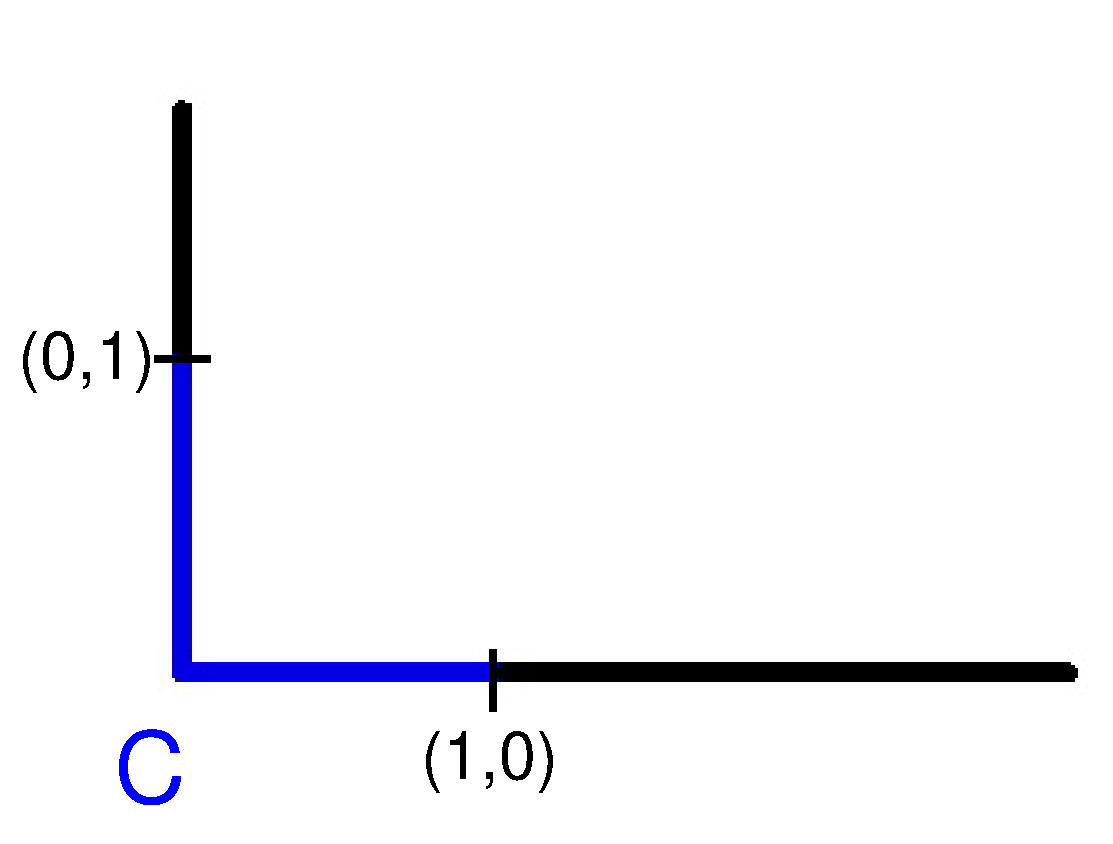
\includegraphics[width=4cm]{esquina}
\]

\vspace{2cm}

Probar que
$$
\sigma(t):=
\begin{cases}
\big(0,(1-t)^2\big),\quad&\mbox{si }0\le t\le 1,\\
\big((t-1)^2,0\big),\quad&\mbox{si }1\le t\le 2
\end{cases}
$$
es una parametrizaci\'on $C^1$ de la curva $\C$.

Observar que $\C$ no tiene recta tangente en el $(0,0)$. \textquestiondown Por qu\'e no hay contradicci\'on?
\eej

\bej Sea $\sigma(t)=(t^3,t^3)$ con $-1\le t\le 1$. %Aqu\'{\i}
%$$
%\mbox{signo\,}t=
%\begin{cases}
%-1\quad&\mbox{si\ }t\le0,\\
%\ \ 0\quad&\mbox{si\ }t=0,\\
%\ \ 1\quad&\mbox{si\ }t\ge0,
%\end{cases}
%$$
%
%\begin{center}
%\includegraphics[width=5cm]{signo}
%\end{center}

Probar que $\sigma$ es una parametrizaci\'on $C^1$ del segmento $y=x$, $-1\le x\le 1$ que es una curva suave.

Observar que $\sigma'(0)=(0,0)$.
\eej


\bej Sea $\C$ el arco de par\'abola $y=x^2$ con $0\le x\le1$.
\begin{enumerate}
\item[a).] Probar que $\C$ es una curva abierta, simple, suave
\item[b).] Probar que $\bar \sigma(s):=\big(\bar x(s),\bar y(s)\big)$ dada por
$$
\left\{
\begin{aligned}
& \bar x(s)=e^s-1\\
&\hskip4cm 0\le s\le \mbox{ln\,}2\\
&\bar y(s)=(e^s-1)^2
\end{aligned}
\right.
$$
es una parametrizací\'on regular de $\C$.

\item[c).] Observar que $\sigma(t):=(t,t^2)$ con $t\in[0,1]$ es otra parametrizaci\'on regular.

\item[d).] Hallar una funci\'on $g:[0,1]\to[0,\mbox{ln\,}2]$ tal que $\bar\sigma\big(g(t)\big)=\sigma(t)$ para todo
$t\in[0,1]$.

Observar que $g$ es biyectiva y $C^1$.
\end{enumerate}
\eej

%Ejercicio suproimido 1C 2016
%\bej Sea $\C$ una curva cerrada, simple, suave y $\sigma:[a,b]\to
%\R^3$ una parametrizaci\'on regular de $\C$. Sean $\bar a\in(a,b)$
%y $\bar b=\bar a+b-a$. Consideremos la funci\'on $\bar\sigma:[\bar
%a,\bar b]\to\R^3$ definida por
%$$
%\bar\sigma(s)=
%\begin{cases}
%\sigma(s)\quad&\mbox{si\ }s\in[\bar a,b],\\
%\sigma\big(a+(s-b))\big)&\mbox{si\ }s\in[b,\bar b].
%\end{cases}
%$$


%\begin{enumerate}
%\item
%Probar que $\bar\sigma$ es una parametrizaci\'on regular de
%$\C$ (que recorre la curva $\C$ desde y hasta el punto
%$\sigma(\bar a)$).

%\item Probar que $\bar\sigma$ es una reparametrizaci\'on de
%$\sigma$ (que recorre la curva $\C$ desde y hasta el punto
%$\sigma(\bar a)$).
%\end{enumerate}

%\eej

%Ejercicio suproimido 1C 2016
%\bej Sea $\C$ una curva simple, suave. Sea $\sigma:[a,b]\to\R^3$ una parametrizaci\'on regular de $\C$.
%Sea $[a_1,  b_1]$ un intervalo arbitrario. Consideremos la funci\'on $\sigma_1:[ a_1, b_1]\to\R^3$ definida
%por
%$$
%\sigma_1(s)=\sigma\Big(a+\frac{b-a}{b_1- a_1}(s- a_1)\Big).
%$$
%Probar que $\sigma_1$ es una parametrizaci\'on regular de $\C$.

%\eej

\bigskip


\noindent{\Large\bf {Integral de longitud de arco}}

\bej Considere la curva definida por \(\sigma(t) = (t - \sen t, 1 - \cos t)\). Calcular \(\sigma'(t)\), la norma \(\|\sigma'(t)\|\), y la longitud del arco entre los puntos \(\sigma(0)\) y \(\sigma(2\pi)\). Observe que \(\sigma\) describe la posición de un punto en el borde de un círculo de radio \(1\) que rueda sin deslizar. Esta curva es conocida como cicloide.

\eej

\bej  En los siguientes  casos, calcular la longitud  de la curva, donde $\sigma$ es una parametrización de la misma
sobre el intervalo $[a,b]$, siendo:

\begin{enumerate}
\item[a)]  $\sigma(t)=(t,t^2),\, a=0, \, b=1.$

\item[b)]  $\sigma(t)=(\sqrt{t},t+1,t),\, a=10, \, b=20.$ \bigskip
\end{enumerate}
\eej

\bej Sea \( C \) una curva simple, suave, y sea \( \sigma: [a, b] \to \mathbb{R}^3 \) una parametrización regular de \( C \). Definimos la longitud del arco de curva entre los puntos \( \sigma(a) \) y \( \sigma(t) \) como  
\[
g(t) = \int_a^t \|\sigma'(\tau)\| \, d\tau, \quad t \in [a, b].
\] 
\begin{enumerate}
    \item Demostrar que la función \( g(t) \) es $C^1$ y calcular su derivada. Deducir que $g$ es inversible y que su inversa es de clase $C^1$.  
    \item Considerando \( \ell = g(b) \), definir la nueva parametrización  
    \[
    \tilde{\sigma}(s) = \sigma(g^{-1}(s)), \quad s \in [0, \ell],
    \]  
    y demostrar que \( \tilde{\sigma} \) es una parametrización regular de \( C \).
    \item Probar que la longitud del arco entre los puntos \( \tilde{\sigma}(0) \) y \( \tilde{\sigma}(s) \) es igual a \( s \), para todo \( s \in [0, \ell] \).
\end{enumerate}

\noindent Esto justifica el uso de la notación \( ds \) para denotar el diferencial de la longitud de arco.
\eej

%Ejercicio suproimido 1C 2016
%\bej Sea $\C$ la curva dada por
%$$\left\{
%\begin{aligned}
%&x=a \cos t\\
%&y=a\sen t\qquad t>0.\\
%&z=b\,t
%\end{aligned}
%\right.$$
%Parametrizar esta curva por longitud de arco.
%\eej

\bej  Evaluar las  integrales de longitud de arco $\int_\C
f(x,y,z)\,ds$, donde $\sigma$ es una parametrización de $\C$, en los casos siguientes:

\begin{enumerate}
\item[a).]  $f(x,y,z)=x+y+z,\quad \sigma (t)= (\mbox{sen} t,\cos t,t),\quad t\in
[0,2\pi ].$

\item[b).]  $f(x,y,z)=\cos z,\quad \sigma $ como en la parte 1.

\item[c).]  $f(x,y,z)=x\cos z,\quad \sigma (t)= (t,t^2,0),\quad t\in [0,1].$
\end{enumerate}
\eej

\bej

\begin{enumerate}
\item[a).]
Mostrar que la integral de longitud de arco de $f(x,y)$ a lo largo de una
curva dada en coordenadas polares por $r=r(\theta )$, $\theta _1\leq
\theta \leq \theta _2$ es
\[
\int_{\theta _1}^{\theta _2}f(r\cos \theta ,r\sin \theta )\sqrt{r^2+\left(
\frac{dr}{d\theta }\right) ^2}\,d\theta .
\]

\item[b).]  Calcular la longitud de la curva $r=1+\cos \theta $, $0\leq \theta
\leq 2\pi $. \bigskip
\end{enumerate}
\eej


\bej  Suponer que la semicircunferencia parametrizado por:
\[
\sigma (\theta)= (0,a\,\mbox{sen\,} \theta ,a\cos \theta
),\qquad \theta\in[0,\pi ],
\]
con $a>0$, est\'{a} hecha de alambre con densidad uniforme de 2 gramos por unidad de
longitud.
\begin{enumerate}
\item[a).]  \textquestiondown Cu\'{a}l es la masa total del alambre?
\item[b).]  Si la temperatura ambiente es igual a $x+y-z$ en el punto $(x,y,z)$, calcular la temperatura
promedio sobre el alambre.
\end{enumerate}
\eej

\bej  Si $f:[a,b]\to \mathbb{R}$ es continuamente diferenciable a trozos,
 el gr\'{a}fico de $f$ en $[a,b]$ es una curva que se puede parametrizar como $\sigma(t)= (t,f(t))$ para $t\in [a,b]$.


\begin{enumerate}
\item[a).]  Mostrar que la longitud del gr\'{a}fico de $f$ en [a,b] es
\[
\int^b_a\sqrt{1+[f^{\prime }(x)]^2}\,dx.
\]

\item[b).]  Hallar la longitud del  gr\'{a}fico de $y=\log x$ de $x=1$ a $x=2$.
\end{enumerate}
\eej

%Ejercicio suproimido 1C 2016
%\bej Se quiere pintar una cerca que se encuentra sobre un campo
%ondulado. La cerca se encuentra a una distancia variable de una ruta recta que
%supondremos que ocupa el eje y.

%Pongamos el kil\'ometro 0 de la ruta a la altura del comienzo de la cerca. Esta se encuentra
%entre los kil\'ometros 0 y 1, a una distancia variable igual a $ y(1- y)+1$  del kil\'ometro $y$ de la ruta
%(calculada sobre el plano del nivel del mar).

%El terreno puede describirse por medio de su altura sobre el nivel del mar. Con ese fin, describiremos el plano del
%nivel del mar en t\'erminos de la distancia $x$ (en kilómetros) desde el punto a la ruta (sobre el plano) y del
%kilometraje $y$ que le corresponde sobre la ruta. En estos t\'erminos, la altura $z$ del terreno sobre el nivel del mar en los puntos %$(x,y)$
%cercanos a la cerca es $(1- y)+x$.

%Nuestra cerca tiene altura variable $h=\frac{1+y}{750}$ a la altura del  kil\'ometro
%$y$ de la ruta si $0\le y\le 1/2$ y $h=\frac{2-y}{750}$ si $1/2\le y\le 1$.

%Si 1 litro de pintura rinde $4\, m^2$, \textquestiondown cu\'antos litros de pintura tengo que comprar?

%\eej

\bigskip\bigskip

\noindent{\Large\bf {Integrales curvilíneas}}

\bej  Sea ${\bf F}(x,y,z)=(x,y,z)$. Evaluar la integral curvilínea de ${\bf F}$ a lo
largo de las curvas orientadas $\C$ dadas por las siguientes parametrizaciones:

\begin{enumerate}
\item[a).]  $\sigma (t)=(t,t,t),\quad 0\leq t\leq 1.$

\item[b).]  $\sigma(t) =(\sin t,0,\cos t),\quad 0\leq t\leq 2\pi. $
\end{enumerate}
\eej

\bej Para las curvas orientadas $\C$ parametrizadas por las correspondientes funciones $\sigma$,
evaluar las integrales siguientes:

\begin{enumerate}
\item[a).]  $\int_\C x\,dy-y\,dx,\quad \sigma(t) =(\cos t,\sin t),\quad 0\leq
t\leq 2\pi. $

\item[b).]  $\int_\C x\,dx+y\,dy,\quad \sigma(t) =(\cos (\pi t),\sin (\pi
t)),\quad 0\leq t\leq 2.$
\end{enumerate}
\eej

\bej  Considerar la fuerza ${\bf F}(x,y,z)=(x,y,z)$. Calcular el trabajo
realizado al mover una part\'{\i }cula a lo largo de la par\'{a}bola $%
y=x^2,\,z=0$, de $x=-1$ a $x=2$.
\eej

\bej  Sea $\C $ una curva orientada suave parametrizada por  $\sigma$.
\begin{enumerate}
\item[a).] Suponer que ${\bf F}$ es
perpendicular a {$\sigma $}$^{\prime }(t)$ en $\sigma(t) $ para todo $t$. Mostrar que
\[
\int_\C {\bf F}\cdot d{\bf s}=0.
\]

\item[b).]  Si ${\bf F}$ es paralelo a {$\sigma $}$^{\prime }(t)$ en $\sigma(t) $ para todo $t$,
mostrar que
\[
\int_\C {\bf F}\cdot d{\bf s}=\int_\C ||{\bf F}||\,ds.
\]
(Aquí, por paralelo a $\sigma ^{\prime }(t)$ se entiende que ${\bf F}\big(\sigma(t)\big
)=\lambda (t)${$\sigma $}$^{\prime }(t)$, donde $\lambda (t)>0$.)
\end{enumerate}

\eej

\bej  \textquestiondown Cu\'{a}l es el valor de la integral curvilínea de un campo
gradiente sobre una curva cerrada $C$?
\eej

\bej  Suponer que $\nabla f(x,y,z)=(2xyze^{x^2},ze^{x^2},ye^{x^2})$. Si $%
f(0,0,0)=5$, hallar $f(1,1,2)$.
\eej

\bej  Considerar el campo de fuerza gravitacional (con $G=m=M=1$) definido
(para $(x,y,z)\neq (0,0,0)$) por:
\[
{\bf F}(x,y,z)={\frac{-1}{(x^2+y^2+z^2)^{\frac 32}}}(x,y,z).
\]
Mostrar que el trabajo realizado por la fuerza gravitacional conforme una
part\'{\i }cula se mueve de $(x_1,y_1,z_1)$ a $(x_2,y_2,z_2)$, a lo largo de
cualquier trayectoria, depende solamente de los radios $R_1=\sqrt{%
x_1^2+y_1^2+z_1^2}$ y $R_2=\sqrt{x_2^2+y_2^2+z_2^2}$.
\eej

\bej
Considere la curva $C = \{(x, y, z) \in \mathbb{R}^3 : y = 1 - x^2, \, x + y + z = 1, \, x \geq 0, \, y \geq 0 \}$.

\begin{enumerate}
    \item[a)] Obtenga una parametrización regular de $C$ que comience en $(0, 1, 0)$ y termine en $(1, 0, 0)$.
    \item[b)] Calcule la integral $\int_C \mathbf{F} \cdot d\mathbf{s}$ con $C$ orientada como en a), donde $\mathbf{F}(x, y, z) = (2x, y, -z)$.
\end{enumerate}
\eej


\bej Sean $f:\R^3\to\R$ una función $C^1$,  $\textbf{G}:\R^3\to\R^3$ un campo $C^1$ y
$\textbf{F}=\nabla f+\textbf{G}$. Sea
$\C$ una curva cerrada, simple, suave, orientada. Verificar que
$$
\int_\C \textbf{F}\cdot d\textbf{s}=\int_\C \textbf{G}\cdot d\textbf{s}.
$$
\eej

\bej Sea $\C$ una curva suave, $\sigma:[a,b]\to\R^3$ una parametrización regular de $\C$. Sea $g:[\bar a,\bar b]\to[a,b]$
una biyección $C^1$ con $g'(\tau)\neq0$ para todo $\tau\in[a,b]$. Sea $\bar\sigma:[\bar a,\bar b]\to\R^3$  dada por
 $\bar\sigma(s)=\sigma\big(g(s)\big)$. Llamamos a $\bar
\sigma$ una \bf {reparametrización} de $\sigma$.
\begin{enumerate}
\item[a).] Probar que $\bar \sigma$ es una parametrización regular de $\C$.

\item[b).] Sea $f:\R^3\to \R$ continua. Ver que el cálculo de $\int_\C f\,ds$ da el mismo resultado cuando la integral
se evalúa utilizando la parametrización $\sigma$ o la parametrización $\bar\sigma$.

\item[c).] Sea ${\bf F}:\R^3\to\R^3$ continua. Suponer que orientamos a $\C$ con la orientación dada por $\sigma$. Ver que el
cálculo de $\int_\C {\bf F}\cdot d{\bf s}$ utilizando la parametrización $\bar\sigma$ da el mismo resultado que
cuando se utiliza $\sigma$, si
$\bar\sigma$ preserva la orientación de $\C$. Ver que si no es así, los resultados difieren sólo en el signo.

\end{enumerate}
\eej

\end{document}
